\documentclass[10pt]{article}
\usepackage{tmlr}
%%%%% NEW MATH DEFINITIONS %%%%%

\usepackage{amsmath,amsfonts,bm}

% Mark sections of captions for referring to divisions of figures
\newcommand{\figleft}{{\em (Left)}}
\newcommand{\figcenter}{{\em (Center)}}
\newcommand{\figright}{{\em (Right)}}
\newcommand{\figtop}{{\em (Top)}}
\newcommand{\figbottom}{{\em (Bottom)}}
\newcommand{\captiona}{{\em (a)}}
\newcommand{\captionb}{{\em (b)}}
\newcommand{\captionc}{{\em (c)}}
\newcommand{\captiond}{{\em (d)}}

% Highlight a newly defined term
\newcommand{\newterm}[1]{{\bf #1}}


% Figure reference, lower-case.
\def\figref#1{figure~\ref{#1}}
% Figure reference, capital. For start of sentence
\def\Figref#1{Figure~\ref{#1}}
\def\twofigref#1#2{figures \ref{#1} and \ref{#2}}
\def\quadfigref#1#2#3#4{figures \ref{#1}, \ref{#2}, \ref{#3} and \ref{#4}}
% Section reference, lower-case.
\def\secref#1{section~\ref{#1}}
% Section reference, capital.
\def\Secref#1{Section~\ref{#1}}
% Reference to two sections.
\def\twosecrefs#1#2{sections \ref{#1} and \ref{#2}}
% Reference to three sections.
\def\secrefs#1#2#3{sections \ref{#1}, \ref{#2} and \ref{#3}}
% Reference to an equation, lower-case.
\def\eqref#1{equation~\ref{#1}}
% Reference to an equation, upper case
\def\Eqref#1{Equation~\ref{#1}}
% A raw reference to an equation---avoid using if possible
\def\plaineqref#1{\ref{#1}}
% Reference to a chapter, lower-case.
\def\chapref#1{chapter~\ref{#1}}
% Reference to an equation, upper case.
\def\Chapref#1{Chapter~\ref{#1}}
% Reference to a range of chapters
\def\rangechapref#1#2{chapters\ref{#1}--\ref{#2}}
% Reference to an algorithm, lower-case.
\def\algref#1{algorithm~\ref{#1}}
% Reference to an algorithm, upper case.
\def\Algref#1{Algorithm~\ref{#1}}
\def\twoalgref#1#2{algorithms \ref{#1} and \ref{#2}}
\def\Twoalgref#1#2{Algorithms \ref{#1} and \ref{#2}}
% Reference to a part, lower case
\def\partref#1{part~\ref{#1}}
% Reference to a part, upper case
\def\Partref#1{Part~\ref{#1}}
\def\twopartref#1#2{parts \ref{#1} and \ref{#2}}

\def\ceil#1{\lceil #1 \rceil}
\def\floor#1{\lfloor #1 \rfloor}
\def\1{\bm{1}}
\newcommand{\train}{\mathcal{D}}
\newcommand{\valid}{\mathcal{D_{\mathrm{valid}}}}
\newcommand{\test}{\mathcal{D_{\mathrm{test}}}}

\def\eps{{\epsilon}}


% Random variables
\def\reta{{\textnormal{$\eta$}}}
\def\ra{{\textnormal{a}}}
\def\rb{{\textnormal{b}}}
\def\rc{{\textnormal{c}}}
\def\rd{{\textnormal{d}}}
\def\re{{\textnormal{e}}}
\def\rf{{\textnormal{f}}}
\def\rg{{\textnormal{g}}}
\def\rh{{\textnormal{h}}}
\def\ri{{\textnormal{i}}}
\def\rj{{\textnormal{j}}}
\def\rk{{\textnormal{k}}}
\def\rl{{\textnormal{l}}}
% rm is already a command, just don't name any random variables m
\def\rn{{\textnormal{n}}}
\def\ro{{\textnormal{o}}}
\def\rp{{\textnormal{p}}}
\def\rq{{\textnormal{q}}}
\def\rr{{\textnormal{r}}}
\def\rs{{\textnormal{s}}}
\def\rt{{\textnormal{t}}}
\def\ru{{\textnormal{u}}}
\def\rv{{\textnormal{v}}}
\def\rw{{\textnormal{w}}}
\def\rx{{\textnormal{x}}}
\def\ry{{\textnormal{y}}}
\def\rz{{\textnormal{z}}}

% Random vectors
\def\rvepsilon{{\mathbf{\epsilon}}}
\def\rvtheta{{\mathbf{\theta}}}
\def\rva{{\mathbf{a}}}
\def\rvb{{\mathbf{b}}}
\def\rvc{{\mathbf{c}}}
\def\rvd{{\mathbf{d}}}
\def\rve{{\mathbf{e}}}
\def\rvf{{\mathbf{f}}}
\def\rvg{{\mathbf{g}}}
\def\rvh{{\mathbf{h}}}
\def\rvu{{\mathbf{i}}}
\def\rvj{{\mathbf{j}}}
\def\rvk{{\mathbf{k}}}
\def\rvl{{\mathbf{l}}}
\def\rvm{{\mathbf{m}}}
\def\rvn{{\mathbf{n}}}
\def\rvo{{\mathbf{o}}}
\def\rvp{{\mathbf{p}}}
\def\rvq{{\mathbf{q}}}
\def\rvr{{\mathbf{r}}}
\def\rvs{{\mathbf{s}}}
\def\rvt{{\mathbf{t}}}
\def\rvu{{\mathbf{u}}}
\def\rvv{{\mathbf{v}}}
\def\rvw{{\mathbf{w}}}
\def\rvx{{\mathbf{x}}}
\def\rvy{{\mathbf{y}}}
\def\rvz{{\mathbf{z}}}

% Elements of random vectors
\def\erva{{\textnormal{a}}}
\def\ervb{{\textnormal{b}}}
\def\ervc{{\textnormal{c}}}
\def\ervd{{\textnormal{d}}}
\def\erve{{\textnormal{e}}}
\def\ervf{{\textnormal{f}}}
\def\ervg{{\textnormal{g}}}
\def\ervh{{\textnormal{h}}}
\def\ervi{{\textnormal{i}}}
\def\ervj{{\textnormal{j}}}
\def\ervk{{\textnormal{k}}}
\def\ervl{{\textnormal{l}}}
\def\ervm{{\textnormal{m}}}
\def\ervn{{\textnormal{n}}}
\def\ervo{{\textnormal{o}}}
\def\ervp{{\textnormal{p}}}
\def\ervq{{\textnormal{q}}}
\def\ervr{{\textnormal{r}}}
\def\ervs{{\textnormal{s}}}
\def\ervt{{\textnormal{t}}}
\def\ervu{{\textnormal{u}}}
\def\ervv{{\textnormal{v}}}
\def\ervw{{\textnormal{w}}}
\def\ervx{{\textnormal{x}}}
\def\ervy{{\textnormal{y}}}
\def\ervz{{\textnormal{z}}}

% Random matrices
\def\rmA{{\mathbf{A}}}
\def\rmB{{\mathbf{B}}}
\def\rmC{{\mathbf{C}}}
\def\rmD{{\mathbf{D}}}
\def\rmE{{\mathbf{E}}}
\def\rmF{{\mathbf{F}}}
\def\rmG{{\mathbf{G}}}
\def\rmH{{\mathbf{H}}}
\def\rmI{{\mathbf{I}}}
\def\rmJ{{\mathbf{J}}}
\def\rmK{{\mathbf{K}}}
\def\rmL{{\mathbf{L}}}
\def\rmM{{\mathbf{M}}}
\def\rmN{{\mathbf{N}}}
\def\rmO{{\mathbf{O}}}
\def\rmP{{\mathbf{P}}}
\def\rmQ{{\mathbf{Q}}}
\def\rmR{{\mathbf{R}}}
\def\rmS{{\mathbf{S}}}
\def\rmT{{\mathbf{T}}}
\def\rmU{{\mathbf{U}}}
\def\rmV{{\mathbf{V}}}
\def\rmW{{\mathbf{W}}}
\def\rmX{{\mathbf{X}}}
\def\rmY{{\mathbf{Y}}}
\def\rmZ{{\mathbf{Z}}}

% Elements of random matrices
\def\ermA{{\textnormal{A}}}
\def\ermB{{\textnormal{B}}}
\def\ermC{{\textnormal{C}}}
\def\ermD{{\textnormal{D}}}
\def\ermE{{\textnormal{E}}}
\def\ermF{{\textnormal{F}}}
\def\ermG{{\textnormal{G}}}
\def\ermH{{\textnormal{H}}}
\def\ermI{{\textnormal{I}}}
\def\ermJ{{\textnormal{J}}}
\def\ermK{{\textnormal{K}}}
\def\ermL{{\textnormal{L}}}
\def\ermM{{\textnormal{M}}}
\def\ermN{{\textnormal{N}}}
\def\ermO{{\textnormal{O}}}
\def\ermP{{\textnormal{P}}}
\def\ermQ{{\textnormal{Q}}}
\def\ermR{{\textnormal{R}}}
\def\ermS{{\textnormal{S}}}
\def\ermT{{\textnormal{T}}}
\def\ermU{{\textnormal{U}}}
\def\ermV{{\textnormal{V}}}
\def\ermW{{\textnormal{W}}}
\def\ermX{{\textnormal{X}}}
\def\ermY{{\textnormal{Y}}}
\def\ermZ{{\textnormal{Z}}}

% Vectors
\def\vzero{{\bm{0}}}
\def\vone{{\bm{1}}}
\def\vmu{{\bm{\mu}}}
\def\vtheta{{\bm{\theta}}}
\def\va{{\bm{a}}}
\def\vb{{\bm{b}}}
\def\vc{{\bm{c}}}
\def\vd{{\bm{d}}}
\def\ve{{\bm{e}}}
\def\vf{{\bm{f}}}
\def\vg{{\bm{g}}}
\def\vh{{\bm{h}}}
\def\vi{{\bm{i}}}
\def\vj{{\bm{j}}}
\def\vk{{\bm{k}}}
\def\vl{{\bm{l}}}
\def\vm{{\bm{m}}}
\def\vn{{\bm{n}}}
\def\vo{{\bm{o}}}
\def\vp{{\bm{p}}}
\def\vq{{\bm{q}}}
\def\vr{{\bm{r}}}
\def\vs{{\bm{s}}}
\def\vt{{\bm{t}}}
\def\vu{{\bm{u}}}
\def\vv{{\bm{v}}}
\def\vw{{\bm{w}}}
\def\vx{{\bm{x}}}
\def\vy{{\bm{y}}}
\def\vz{{\bm{z}}}

% Elements of vectors
\def\evalpha{{\alpha}}
\def\evbeta{{\beta}}
\def\evepsilon{{\epsilon}}
\def\evlambda{{\lambda}}
\def\evomega{{\omega}}
\def\evmu{{\mu}}
\def\evpsi{{\psi}}
\def\evsigma{{\sigma}}
\def\evtheta{{\theta}}
\def\eva{{a}}
\def\evb{{b}}
\def\evc{{c}}
\def\evd{{d}}
\def\eve{{e}}
\def\evf{{f}}
\def\evg{{g}}
\def\evh{{h}}
\def\evi{{i}}
\def\evj{{j}}
\def\evk{{k}}
\def\evl{{l}}
\def\evm{{m}}
\def\evn{{n}}
\def\evo{{o}}
\def\evp{{p}}
\def\evq{{q}}
\def\evr{{r}}
\def\evs{{s}}
\def\evt{{t}}
\def\evu{{u}}
\def\evv{{v}}
\def\evw{{w}}
\def\evx{{x}}
\def\evy{{y}}
\def\evz{{z}}

% Matrix
\def\mA{{\bm{A}}}
\def\mB{{\bm{B}}}
\def\mC{{\bm{C}}}
\def\mD{{\bm{D}}}
\def\mE{{\bm{E}}}
\def\mF{{\bm{F}}}
\def\mG{{\bm{G}}}
\def\mH{{\bm{H}}}
\def\mI{{\bm{I}}}
\def\mJ{{\bm{J}}}
\def\mK{{\bm{K}}}
\def\mL{{\bm{L}}}
\def\mM{{\bm{M}}}
\def\mN{{\bm{N}}}
\def\mO{{\bm{O}}}
\def\mP{{\bm{P}}}
\def\mQ{{\bm{Q}}}
\def\mR{{\bm{R}}}
\def\mS{{\bm{S}}}
\def\mT{{\bm{T}}}
\def\mU{{\bm{U}}}
\def\mV{{\bm{V}}}
\def\mW{{\bm{W}}}
\def\mX{{\bm{X}}}
\def\mY{{\bm{Y}}}
\def\mZ{{\bm{Z}}}
\def\mBeta{{\bm{\beta}}}
\def\mPhi{{\bm{\Phi}}}
\def\mLambda{{\bm{\Lambda}}}
\def\mSigma{{\bm{\Sigma}}}

% Tensor
\DeclareMathAlphabet{\mathsfit}{\encodingdefault}{\sfdefault}{m}{sl}
\SetMathAlphabet{\mathsfit}{bold}{\encodingdefault}{\sfdefault}{bx}{n}
\newcommand{\tens}[1]{\bm{\mathsfit{#1}}}
\def\tA{{\tens{A}}}
\def\tB{{\tens{B}}}
\def\tC{{\tens{C}}}
\def\tD{{\tens{D}}}
\def\tE{{\tens{E}}}
\def\tF{{\tens{F}}}
\def\tG{{\tens{G}}}
\def\tH{{\tens{H}}}
\def\tI{{\tens{I}}}
\def\tJ{{\tens{J}}}
\def\tK{{\tens{K}}}
\def\tL{{\tens{L}}}
\def\tM{{\tens{M}}}
\def\tN{{\tens{N}}}
\def\tO{{\tens{O}}}
\def\tP{{\tens{P}}}
\def\tQ{{\tens{Q}}}
\def\tR{{\tens{R}}}
\def\tS{{\tens{S}}}
\def\tT{{\tens{T}}}
\def\tU{{\tens{U}}}
\def\tV{{\tens{V}}}
\def\tW{{\tens{W}}}
\def\tX{{\tens{X}}}
\def\tY{{\tens{Y}}}
\def\tZ{{\tens{Z}}}


% Graph
\def\gA{{\mathcal{A}}}
\def\gB{{\mathcal{B}}}
\def\gC{{\mathcal{C}}}
\def\gD{{\mathcal{D}}}
\def\gE{{\mathcal{E}}}
\def\gF{{\mathcal{F}}}
\def\gG{{\mathcal{G}}}
\def\gH{{\mathcal{H}}}
\def\gI{{\mathcal{I}}}
\def\gJ{{\mathcal{J}}}
\def\gK{{\mathcal{K}}}
\def\gL{{\mathcal{L}}}
\def\gM{{\mathcal{M}}}
\def\gN{{\mathcal{N}}}
\def\gO{{\mathcal{O}}}
\def\gP{{\mathcal{P}}}
\def\gQ{{\mathcal{Q}}}
\def\gR{{\mathcal{R}}}
\def\gS{{\mathcal{S}}}
\def\gT{{\mathcal{T}}}
\def\gU{{\mathcal{U}}}
\def\gV{{\mathcal{V}}}
\def\gW{{\mathcal{W}}}
\def\gX{{\mathcal{X}}}
\def\gY{{\mathcal{Y}}}
\def\gZ{{\mathcal{Z}}}

% Sets
\def\sA{{\mathbb{A}}}
\def\sB{{\mathbb{B}}}
\def\sC{{\mathbb{C}}}
\def\sD{{\mathbb{D}}}
% Don't use a set called E, because this would be the same as our symbol
% for expectation.
\def\sF{{\mathbb{F}}}
\def\sG{{\mathbb{G}}}
\def\sH{{\mathbb{H}}}
\def\sI{{\mathbb{I}}}
\def\sJ{{\mathbb{J}}}
\def\sK{{\mathbb{K}}}
\def\sL{{\mathbb{L}}}
\def\sM{{\mathbb{M}}}
\def\sN{{\mathbb{N}}}
\def\sO{{\mathbb{O}}}
\def\sP{{\mathbb{P}}}
\def\sQ{{\mathbb{Q}}}
\def\sR{{\mathbb{R}}}
\def\sS{{\mathbb{S}}}
\def\sT{{\mathbb{T}}}
\def\sU{{\mathbb{U}}}
\def\sV{{\mathbb{V}}}
\def\sW{{\mathbb{W}}}
\def\sX{{\mathbb{X}}}
\def\sY{{\mathbb{Y}}}
\def\sZ{{\mathbb{Z}}}

% Entries of a matrix
\def\emLambda{{\Lambda}}
\def\emA{{A}}
\def\emB{{B}}
\def\emC{{C}}
\def\emD{{D}}
\def\emE{{E}}
\def\emF{{F}}
\def\emG{{G}}
\def\emH{{H}}
\def\emI{{I}}
\def\emJ{{J}}
\def\emK{{K}}
\def\emL{{L}}
\def\emM{{M}}
\def\emN{{N}}
\def\emO{{O}}
\def\emP{{P}}
\def\emQ{{Q}}
\def\emR{{R}}
\def\emS{{S}}
\def\emT{{T}}
\def\emU{{U}}
\def\emV{{V}}
\def\emW{{W}}
\def\emX{{X}}
\def\emY{{Y}}
\def\emZ{{Z}}
\def\emSigma{{\Sigma}}

% entries of a tensor
% Same font as tensor, without \bm wrapper
\newcommand{\etens}[1]{\mathsfit{#1}}
\def\etLambda{{\etens{\Lambda}}}
\def\etA{{\etens{A}}}
\def\etB{{\etens{B}}}
\def\etC{{\etens{C}}}
\def\etD{{\etens{D}}}
\def\etE{{\etens{E}}}
\def\etF{{\etens{F}}}
\def\etG{{\etens{G}}}
\def\etH{{\etens{H}}}
\def\etI{{\etens{I}}}
\def\etJ{{\etens{J}}}
\def\etK{{\etens{K}}}
\def\etL{{\etens{L}}}
\def\etM{{\etens{M}}}
\def\etN{{\etens{N}}}
\def\etO{{\etens{O}}}
\def\etP{{\etens{P}}}
\def\etQ{{\etens{Q}}}
\def\etR{{\etens{R}}}
\def\etS{{\etens{S}}}
\def\etT{{\etens{T}}}
\def\etU{{\etens{U}}}
\def\etV{{\etens{V}}}
\def\etW{{\etens{W}}}
\def\etX{{\etens{X}}}
\def\etY{{\etens{Y}}}
\def\etZ{{\etens{Z}}}

% The true underlying data generating distribution
\newcommand{\pdata}{p_{\rm{data}}}
% The empirical distribution defined by the training set
\newcommand{\ptrain}{\hat{p}_{\rm{data}}}
\newcommand{\Ptrain}{\hat{P}_{\rm{data}}}
% The model distribution
\newcommand{\pmodel}{p_{\rm{model}}}
\newcommand{\Pmodel}{P_{\rm{model}}}
\newcommand{\ptildemodel}{\tilde{p}_{\rm{model}}}
% Stochastic autoencoder distributions
\newcommand{\pencode}{p_{\rm{encoder}}}
\newcommand{\pdecode}{p_{\rm{decoder}}}
\newcommand{\precons}{p_{\rm{reconstruct}}}

\newcommand{\laplace}{\mathrm{Laplace}} % Laplace distribution

\newcommand{\E}{\mathbb{E}}
\newcommand{\Ls}{\mathcal{L}}
\newcommand{\R}{\mathbb{R}}
\newcommand{\emp}{\tilde{p}}
\newcommand{\lr}{\alpha}
\newcommand{\reg}{\lambda}
\newcommand{\rect}{\mathrm{rectifier}}
\newcommand{\softmax}{\mathrm{softmax}}
\newcommand{\sigmoid}{\sigma}
\newcommand{\softplus}{\zeta}
\newcommand{\KL}{D_{\mathrm{KL}}}
\newcommand{\Var}{\mathrm{Var}}
\newcommand{\standarderror}{\mathrm{SE}}
\newcommand{\Cov}{\mathrm{Cov}}
% Wolfram Mathworld says $L^2$ is for function spaces and $\ell^2$ is for vectors
% But then they seem to use $L^2$ for vectors throughout the site, and so does
% wikipedia.
\newcommand{\normlzero}{L^0}
\newcommand{\normlone}{L^1}
\newcommand{\normltwo}{L^2}
\newcommand{\normlp}{L^p}
\newcommand{\normmax}{L^\infty}

\newcommand{\parents}{Pa} % See usage in notation.tex. Chosen to match Daphne's book.

\DeclareMathOperator*{\argmax}{arg\,max}
\DeclareMathOperator*{\argmin}{arg\,min}

\DeclareMathOperator{\sign}{sign}
\DeclareMathOperator{\Tr}{Tr}
\let\ab\allowbreak

\usepackage{hyperref}
\usepackage{url}
\usepackage{booktabs}
\usepackage{graphicx}

\title{The Review Lottery: Calibrating an Observational Estimator of Peer-Review Noise (ICLR 2017-2025)}

% anonymous submission: author block hidden by tmlr style

\def\month{10}
\def\year{2026}
\def\openreview{\url{https://openreview.net/forum?id=XXXX}}

\begin{document}
\maketitle

\begin{abstract}
How much of a conference accept/reject decision would change if the same paper were reviewed by a different set of reviewers? Running a second independent program committee is the gold standard for answering this, but it is prohibitively expensive: it has been done only twice, at NeurIPS 2014 and NeurIPS 2021. We build an observational estimator of this quantity from public review data alone, calibrate it twice, and apply it to nine years of ICLR (2017--2025; 36,113 papers, 134,912 reviews). The estimator decomposes review scores with a Bayesian ordered-probit model into paper quality and reviewer noise, maps simulated scores to decisions with a logistic model, and simulates two independent committees (posterior draws $B=1{,}000$; committee sizes $k=2$,3,4). Estimated disagreement rates are 23-30\% at $k=2$ and 18-24\% at $k=4$; 30-50\% of accepted papers would be rejected by an independent committee. External calibration: at the NeurIPS 2021 reviewer-count caliber ($k=3$), the simulated 2021 disagreement rate is 23.3\% [21.7\%, 25.0\%], against the reported 23.0\%, a bias of +0.3 percentage points; accept precision and committee correlation agree within 5pp and 0.04. Internal calibration: on 18,740 papers with four or more reviews, random model-free $2{+}2$ reviewer splits agree with the $k=2$ simulation within 1\,pp in 2018 and 2021--2025. Longitudinally, we find no robust time trend in reviewer noise over 2017--2025. The unusually high accepted-paper flip rates of 2020 and 2021 have distinct mechanisms: the 2020 four-point scale compressed scores (23.7\% of papers had zero within-paper variance), and a counterfactual experiment shows coarsening the scale raises disagreement by about 7pp; 2021 instead combined the lowest signal-to-noise ratio in the sample with the most threshold-crowded acceptances. For the LLM era, a 2023 breakpoint test on within-paper score variance finds no break, but the design has almost no power, and no post-2022 review text or confidence data are available, so no attribution to LLMs is attempted.
\end{abstract}

\section{Introduction}

Peer review at large machine learning conferences rests on an uncomfortable fact: the same paper, sent to a different set of reviewers, might receive a different decision. The only direct measurements of this counterfactual come from two randomized experiments. At NeurIPS 2014, 166 papers were reviewed by two independent program committees, which disagreed on 43 papers (25.9\%); about half of accepted papers would have been rejected by the other committee (accept precision 49.5\%), and roughly 50\% of the variation in quality scores was estimated to be subjective in origin \citep{cortes2021}. At NeurIPS 2021, the experiment was repeated at larger scale ($n=882$): the committees disagreed on 23.0\% of papers, with accept precision 50.6\% across committees \citep{beygelzimer2023}. These experiments are the field's only ground truth for review noise, and they cannot be repeated casually: each required duplicating the review of hundreds of papers.

This paper asks whether the same counterfactual quantity can be estimated from observational data alone, and whether such an estimator can be trusted. We make two contributions.

First, we construct an estimator of two-committee disagreement from public review scores. A Bayesian ordered-probit variance decomposition separates each paper's latent quality from reviewer noise, year by year, with year-specific cutpoints absorbing scale changes. A logistic decision model maps simulated scores to accept/reject outcomes, approximating the area-chair stage. Drawing from the posterior, we simulate two independent committees of k reviewers for each paper and record the disagreement rate, the probability that an accepted paper flips, and related quantities. The estimator requires only review scores and final decisions, both public on OpenReview.

Second, we calibrate the estimator twice before trusting it. The external anchor compares simulated disagreement to the reported NeurIPS 2014 and 2021 numbers under matched reviewer-count calibers. The internal anchor is model-free: on ICLR papers with four or more reviews (23,995 papers, 23,678 of them in 2021--2025), we randomly split reviewers into two groups of two, pass each group through the same decision model, and compare the resulting split-half disagreement (200 repetitions) to the $k=2$ simulation. This second check depends on no modeling assumptions about score generation.
%phase1_report.md

We apply the calibrated estimator to ICLR 2017--2025 and report three sets of findings, corresponding to three preregistered research questions. RQ-A asks whether the estimator reproduces the two anchors. RQ-B asks how reviewer noise evolved over nine years during which submissions grew roughly $24$-fold (489 in 2017 to 11,663 in 2025). RQ-C asks, descriptively, whether review behavior changed around 2023, the start of the LLM era.
%phase1_report.md

Our headline results: the estimator passes both calibrations (external bias +0.3\,pp at the matched caliber; internal bias under 1\,pp in six of nine years). The share of latent score variance attributable to paper quality, $\rho$, ranges from 0.38 to 0.58 across years, consistent with the NeurIPS 2014 estimate of about one half. Simulated two-committee disagreement is 23-30\% at $k=2$. We find no robust longitudinal trend in reviewer noise. The 2020 and 2021 anomalies in accepted-paper flip rates trace to different mechanisms: scale compression in 2020 and low signal plus threshold crowding in 2021. On the LLM question, the data do not support a conclusion either way: a 2023 breakpoint test on within-paper score variance finds no break with a design that has almost no power to find one, and no review text or confidence data exist after 2022.

The rest of the paper is organized as follows. Section 2 reviews related work. Section 3 describes the estimator and the two calibrations. Section 4 reports results for the three research questions. Section 5 discusses interpretation and implications. Section 6 states limitations. Section 7 concludes.

\section{Related Work}

\textbf{Randomized audits of peer review.} The NeurIPS 2014 experiment \citep{cortes2021} duplicated review for 166 papers and reported 43 disagreements (25.9\%), accept precision of 49.5\%, and an estimated 50\% subjective share of score variation. The NeurIPS 2021 experiment \citep{beygelzimer2023} scaled the design to 882 papers and found 23.0\% disagreement with 50.6\% accept precision, concluding that inconsistency had not visibly changed since 2014. These are our external calibration targets; unlike these experiments, our estimator needs no duplicated review.

\textbf{Variance decomposition of ICLR reviews.} The closest prior work is Tran et al.~\citep{tran2020}, who analyzed ICLR 2017--2020 with variance decomposition and simulation, and reported institutional bias and a gender gap. Their analysis has no external calibration, no model-free internal anchor, uses Gaussian ANOVA rather than an ordinal model, and ends in 2020. Our work extends the window to 2025, adds dual calibration, and handles year-specific rating scales with ordered-probit cutpoints.

\textbf{Process-centric analyses of peer review.} A recent large-scale study of ICLR 2017--2025 (over 28,000 submissions) examines how disagreement, rebuttals, and review dynamics relate to acceptance ~\citep{acceptance2025}. It is descriptive about the disagreement-to-acceptance mapping; it does not decompose variance, simulate counterfactual committees, or calibrate against experimental anchors. Our contribution is complementary: an estimator of the rerun counterfactual with quantified calibration error.

\textbf{LLM use in peer review.} Liang et al.~\citep{liang2024} developed a corpus-level maximum-likelihood method for estimating the fraction of review text substantially modified by LLMs, reporting 6.5-16.9\% across ICLR 2024, NeurIPS 2023, CoRL 2023, and EMNLP 2023. Our preregistration planned to apply their method at the aggregate level; as documented in Section 4.3, our data lack post-2022 review text, so this estimation was not feasible and we report only behavioral descriptives, without attribution.

\section{Method}

\subsection{Variance decomposition: ordered probit with annual cutpoints}

For paper i in year y with $k_i$ reviews, reviewer j's score $s_{ij}$ is modeled as an ordered-probit discretization of a latent variable:

$s_{ij}$ ~ OrderedProbit($\theta_i$, $c_y$), $\theta_i$ ~ Normal(0, $\sigma^2_{\mathrm{paper},y}$)

where $c_y$ are year-specific cutpoints. The cutpoints absorb differences in rating scales across years: ICLR used a $1$--$10$ scale in 2017--2019 and 2021, a four-point scale $\{1,3,6,8\}$ in 2020, and a six-point scale $\{1,3,5,6,8,10\}$ in 2022--2025 (verified from the observed score values per year). The latent residual variance is fixed at 1, so the signal-to-noise ratio is
%phase3_report.md sec 1.1

$\rho_y$ = $\sigma^2_{\mathrm{paper},y}$ / ($\sigma^2_{\mathrm{paper},y}$ + 1),

the share of latent score variance attributable to paper quality. The location parameter $\mu_y$ is fixed at 0 for identification (a standard constraint when cutpoints are free, since location shifts are absorbed by the cutpoints).
%phase2_report.md sec 1.1

Fitting is done per year with PyMC NUTS (non-centered parameterization, ADVI initialization, tune=1000, draws=1000, 2 chains, target\_accept=0.9) on CPU. A 2023 pilot (500/500 draws) completed in about 8.5 minutes, below the preregistered 6-hour threshold that would have triggered a reduced sampling scheme; the full 1000/1000 fits were therefore run as planned (the largest year, 2025 with 11,513 papers and 46,722 reviews, took 76.7 minutes). All years show zero divergences and split R-hat between 1.00 and 1.01.
%phase2_report.md sec 1.3
%rho_table.csv; phase2_report.md sec 1.3
%rho_table.csv

Data and cohort. The primary data are the public ICLR reviews from the berenslab/iclr-dataset mirror: 36,113 papers and 134,912 reviews for ICLR 2017--2025. Of these, 11,213 papers were accepted, 17,426 rejected, and 7,474 withdrawn (decision unknown); all unknown decisions were verified to be withdrawals, not data corruption. Withdrawn papers with scores enter the variance decomposition (they contribute to theta estimation) but are excluded from decision-model fitting, which requires an observed outcome. The variance decomposition uses papers with at least one scored review (35,617 papers; 496 papers without scores are excluded). Author identifiers (\texttt{author\_ids}, \texttt{authors}) were deleted at load; a column-name scan confirmed no reviewer identity fields, and no cross-paper reviewer linkage is performed, so reviewer stringency is folded into the noise term.
%phase1_report.md
%phase1_report.md
%phase2_report.md sec 1.4
%data/processed/papers.parquet; phase1_report.md sec 4
%phase1_report.md sec 1

Preregistered deviation. The preregistration specified a $\beta\cdot\mathrm{confidence}$ term in the probit mean. The primary data source carries no confidence field (0 of 134,912 reviews non-empty), so the main fit omits it. A sensitivity analysis refits the same model with $\beta\cdot\mathrm{confidence}$ on the PeerSum ICLR subset (2018--2022, which has confidence; 53,732 reviews): including confidence changes $\rho$ by -0.016 to -0.030 with beta approximately -0.14 to -0.22 (higher-confidence reviewers score slightly lower), a 4-7\% relative shift that does not change the magnitude of the conclusions.
%phase1_report.md
%phase1_report.md
%phase2_report.md sec 6

\subsection{Decision model: from scores to accept/reject}

The area-chair stage is approximated by a logistic regression of the binary decision on paper-level score summaries:

$P(\mathrm{accept}\mid\mathrm{mean\_score},\mathrm{sd\_score},\mathrm{year})$ = logistic($\alpha_{\mathrm{year}}$ + $3.37\cdot\mathrm{mean\_score}-0.14\cdot\mathrm{sd\_score}$),

\begin{figure}[t]
\centering
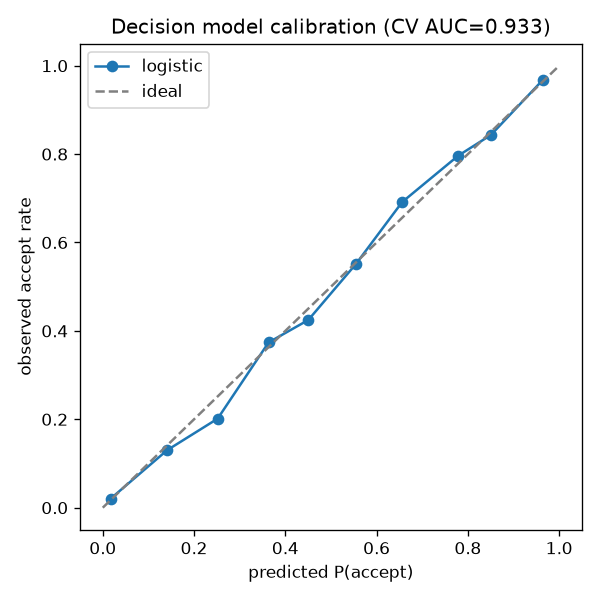
\includegraphics[width=0.62\textwidth]{fig_decision_calibration.png}
\caption{Calibration of the logistic decision model: predicted versus observed acceptance rate (5-fold CV AUC $=0.933$). The model tracks the ideal diagonal closely.}
\label{fig:decision-calib}
\end{figure}
fit on the 28,476 papers with a known decision and scored reviews (5-fold cross-validated AUC 0.933). Higher mean scores raise acceptance odds; higher within-paper score dispersion lowers them, consistent with the descriptive finding that disagreement hurts acceptance ~\citep{acceptance2025}. Year intercepts absorb annual acceptance-rate differences. As a sensitivity check, a pure threshold rule calibrated to each year's acceptance rate was also implemented; the simulation results are consistent across the two rules.
%decision_model_coefs.json; phase2_report.md sec 3
%phase2_report.md sec 3

\subsection{Two-committee simulation}

For each paper with a known decision and scored reviews, the simulation proceeds as follows: (1) draw $\theta_i$ from its posterior; (2) generate two independent sets of k review scores from the fitted ordered-probit model; (3) pass each set through the decision model to obtain two accept/reject decisions; (4) record whether the committees disagree. Posterior draws $B=1{,}000$; k is reported separately for 2, 3, and 4. Summary statistics are the disagreement rate (fraction of papers on which the two committees differ), $P(\mathrm{flip}\mid\mathrm{accepted})$ (fraction of accepted papers the second committee would reject), and $P(\mathrm{flip}\mid\mathrm{rejected})$. The $k=3$ caliber matches the NeurIPS 2021 experiment's reviewer count for external calibration; the $k=2$ caliber matches the internal split-half anchor.
%preregistration_draft.md sec 3.3

\subsection{Dual calibration}

External anchor (NeurIPS randomized experiments). The reported values are: 2014, $43/166 = 25.9\%$ disagreement and approximately 50\% accept precision \citep{cortes2021}; 2021, $203/882 = 23.0\%$ disagreement, 50.6\% accept precision, and committee mean-score correlation 0.575 (initial) / 0.586 (final) \citep{beygelzimer2023}. Because the public NeurIPS data contain only accepted papers, this is a partial calibration by numerical comparison, as preregistered: we compare the simulated quantities at the matched reviewer-count caliber against the reported values and report the bias. The preregistration anticipated the simulated disagreement would be biased downward (the model omits area-chair noise and reviewer-assignment variation); the direction of any bias is reported as found.
%phase0_notes/papers.md
%preregistration_draft.md sec 3.4

Internal anchor (model-free split-half). Among papers with four or more reviews, we randomly split the reviewers into two groups of two, pass each group's scores through the same decision model, and compute the disagreement rate directly, repeating the random split 200 times. This anchor depends on no score-generation model. Its sampling frame is compared against the full paper population to quantify selection bias.
%phase2_report.md sec 5.2

\section{Results}

\subsection{RQ-A: the estimator and its calibration}

\textbf{Variance decomposition.} Paper quality accounts for roughly two-fifths to three-fifths of latent score variance in every year (Table 1). Rho is highest in 2017 (0.583 [0.535, 0.629]) and lowest in 2021 (0.376 [0.356, 0.396]), with the remaining years between 0.410 and 0.481. The magnitude matches the NeurIPS 2014 variance-decomposition estimate of about 50\% subjective variation.
%rho_table.csv
%phase0_notes/papers.md

\begin{figure}[t]
\centering
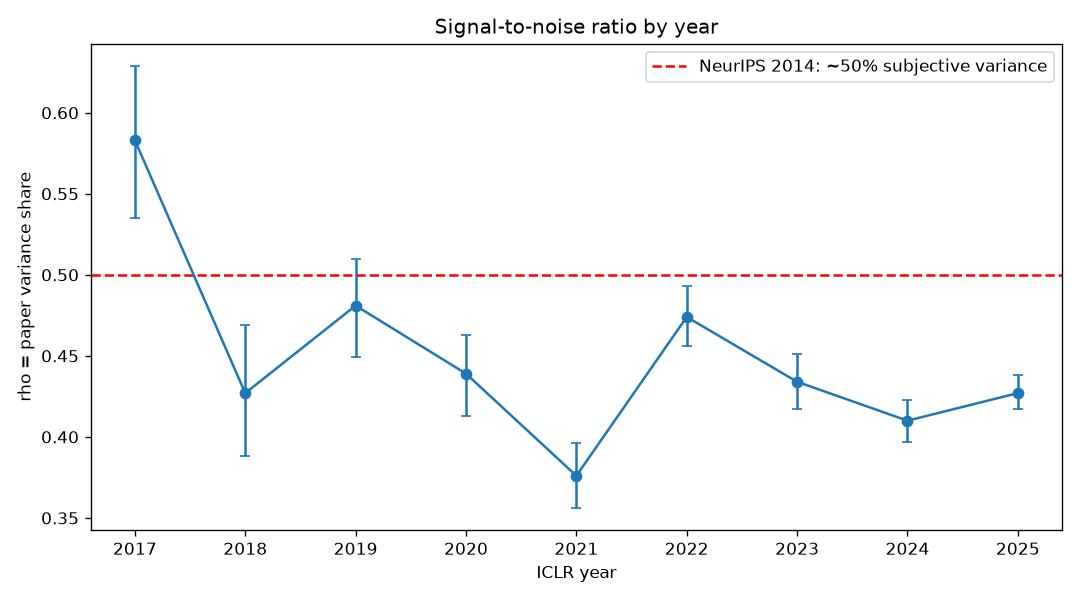
\includegraphics[width=0.85\textwidth]{fig_rho.png}
\caption{Signal-to-noise ratio $\rho_y$ by year (posterior mean, 95\% credible interval). The dashed line marks the NeurIPS 2014 estimate of about 50\% subjective variance.}
\label{fig:rho}
\end{figure}
\begin{table}[t]
\centering
\caption{Signal-to-noise ratio $\rho_y$ by year: posterior mean and 95\% credible interval.}\label{tab:t1}
\begin{tabular}{lrrrr}\toprule
Year & Papers & Reviews & $\rho$ & 95\% CI \\
\midrule
2017 & 489 & 1,508 & 0.583 & [0.535, 0.629] \\
2018 & 969 & 2,921 & 0.427 & [0.388, 0.469] \\
2019 & 1,555 & 4,734 & 0.481 & [0.449, 0.510] \\
2020 & 2,561 & 7,775 & 0.439 & [0.413, 0.463] \\
2021 & 2,974 & 11,488 & 0.376 & [0.356, 0.396] \\
2022 & 3,375 & 13,161 & 0.474 & [0.456, 0.493] \\
2023 & 4,919 & 18,575 & 0.434 & [0.417, 0.451] \\
2024 & 7,262 & 28,028 & 0.410 & [0.397, 0.423] \\
2025 & 11,513 & 46,722 & 0.427 & [0.417, 0.438] \\
\bottomrule
\end{tabular}
\end{table}
% source: rho_table.csv

\textbf{Two-committee simulation.} Replacing the reviewer pool changes the accept/reject decision for roughly one quarter of papers (Table 2). At $k=2$, disagreement ranges from 22.8\% (2017) to 30.3\% (2025); at $k=3$, from 19.7\% to 26.7\%; at $k=4$, from 17.7\% to 24.2\%. Increasing committee size from 2 to 4 reduces disagreement by about 5 percentage points. Among accepted papers, 30-50\% would be rejected by an independent committee; this quantity is highest in 2020 (47.9\%) and 2021 (50.2\%), a pattern examined in Section 4.2.
%sim_summary.csv
%sim_summary.csv

\begin{table}[t]
\centering
\caption{Simulated two-committee disagreement and accepted-paper flip probability, $k=2/3/4$.}\label{tab:t2}
\begin{tabular}{lrrrrr}\toprule
Year & Disagreement $k=2$ & Disagreement $k=3$ & Disagreement $k=4$ & P(flip \ & accepted), $k=2$ \\
\midrule
2017 & 0.228 [0.192, 0.268] & 0.197 & 0.177 & 0.308 \\
2018 & 0.293 [0.263, 0.324] & 0.251 & 0.223 & 0.363 \\
2019 & 0.273 [0.249, 0.297] & 0.231 & 0.203 & 0.344 \\
2020 & 0.268 [0.250, 0.286] & 0.228 & 0.196 & 0.479 \\
2021 & 0.260 [0.244, 0.276] & 0.233 & 0.213 & 0.502 \\
2022 & 0.282 [0.265, 0.300] & 0.249 & 0.224 & 0.352 \\
2023 & 0.293 [0.277, 0.307] & 0.257 & 0.233 & 0.376 \\
2024 & 0.299 [0.288, 0.311] & 0.264 & 0.238 & 0.405 \\
2025 & 0.303 [0.293, 0.313] & 0.267 & 0.242 & 0.384 \\
\bottomrule
\end{tabular}
\end{table}
% source: sim_summary.csv

\begin{figure}[t]
\centering
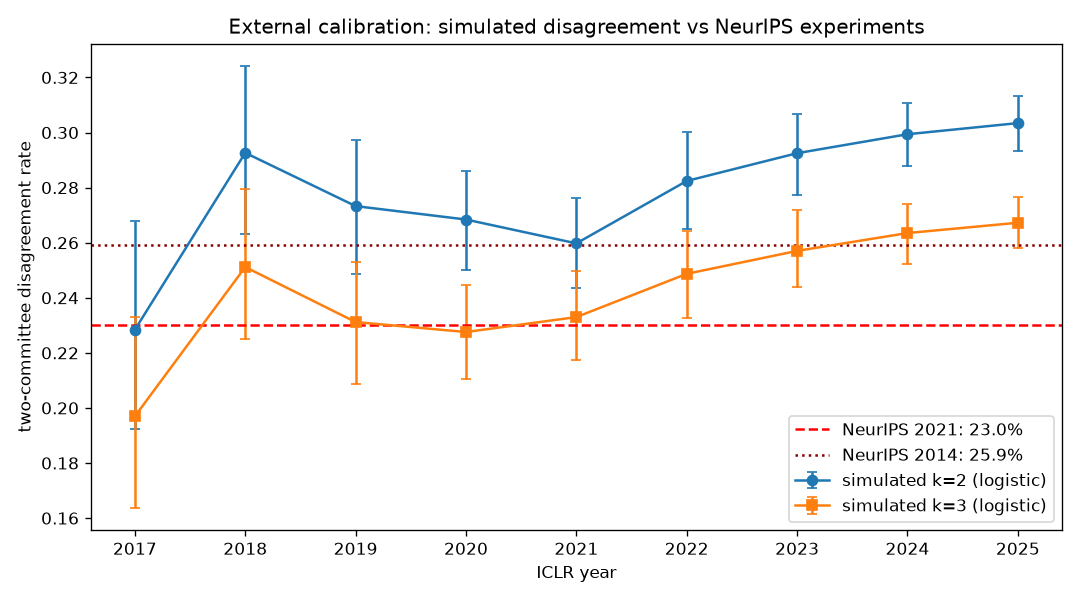
\includegraphics[width=0.85\textwidth]{fig_calib_external.png}
\caption{External calibration: simulated two-committee disagreement at $k=2$ and $k=3$ against the NeurIPS 2014 (25.9\%) and 2021 (23.0\%) experimental values. At the matched $k=3$ caliber the 2021 simulation sits on the observed value.}
\label{fig:calib-external}
\end{figure}
\textbf{External calibration.} At the NeurIPS 2021 reviewer-count caliber ($k=3$), the simulated 2021 disagreement rate is 23.3\% [21.7\%, 25.0\%], against the reported 23.0\%: a bias of +0.3 percentage points, essentially unbiased. The 2014 anchor (25.9\%, $n=166$) is 2.6pp above the same simulated quantity. Accept precision at $k=3$ is simulated at 55.6\% [51.9\%, 59.3\%] versus the reported 50.6\% (+5\,pp); committee mean-score correlation is simulated at 0.618 [0.592, 0.645] versus the reported 0.575/0.586 ($+0.04$). Against the preregistered expectation of downward bias (from omitting area-chair noise), the observed bias is mildly upward but small; the omission of area-chair noise does not produce a systematic underestimate, possibly because reviewer noise in the ICLR data already absorbs most of the assignment variation.
%calib_external.csv; phase0_notes/papers.md
%calib_external.csv; phase0_notes/papers.md
%phase2_report.md sec 5.3

\textbf{Internal calibration.} The model-free split-half anchor (Table 3) agrees with the $k=2$ simulation within 1\,pp in 2018 and in every year from 2021 to 2025, and the pooled split-half rate is 29.6\% [29.2\%, 30.0\%] over 18,740 papers. In 2017, 2019, and 2020 the model sits $3$--$5$\,pp below the anchor (e.g., $-5.4$\,pp in 2017, $-3.2$\,pp in 2020). A plausible explanation is stronger reviewer-assignment homogeneity in the early years: when reviewers within a paper share similar backgrounds, an actual $2{+}2$ split exaggerates between-group differences relative to the model's independent-draws assumption; the coarser 2020 scale may also fit the model slightly worse. From 2021 onward, when reviewer counts and procedures stabilized, the calibration is close. Selection bias in the anchor frame is small: anchor papers average 5.47 versus 5.40 mean score, 40.1\% versus 39.2\% acceptance, and 4.17 versus 3.75 reviews per paper against the full population.
%internal_anchor.json; phase2_report.md sec 5.2
%phase2_report.md sec 5.2

\begin{table}[t]
\centering
\caption{Internal anchor: model-free $2{+}2$ split-half disagreement (200 repetitions) versus the $k=2$ simulation.}\label{tab:t3}
\begin{tabular}{lrrr}\toprule
Year & Split-half & Model $k=2$ & Difference \\
\midrule
2017 & 0.282 [0.205, 0.341] & 0.228 & -0.054 \\
2018 & 0.294 [0.167, 0.444] & 0.293 & -0.001 \\
2019 & 0.321 [0.263, 0.382] & 0.273 & -0.048 \\
2020 & 0.300 [0.266, 0.335] & 0.268 & -0.032 \\
2021 & 0.265 [0.254, 0.276] & 0.260 & -0.005 \\
2022 & 0.287 [0.276, 0.299] & 0.282 & -0.005 \\
2023 & 0.290 [0.282, 0.300] & 0.293 & +0.003 \\
2024 & 0.300 [0.291, 0.308] & 0.299 & -0.001 \\
2025 & 0.307 [0.302, 0.314] & 0.303 & -0.004 \\
\bottomrule
\end{tabular}
\end{table}
% source: internal_anchor.json; phase2_report.md sec 5.2

\begin{figure}[t]
\centering
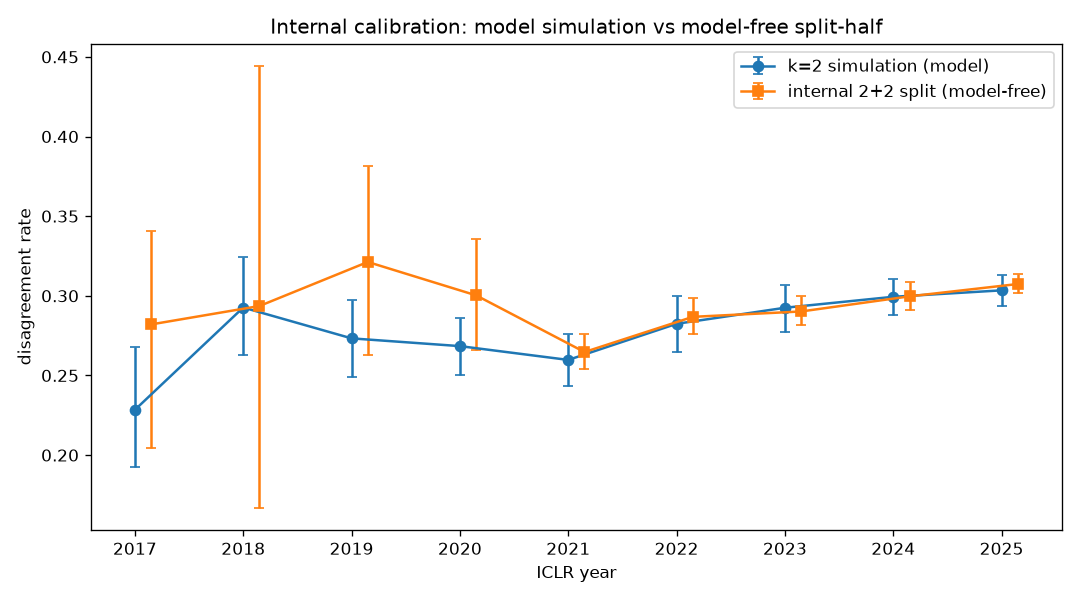
\includegraphics[width=0.85\textwidth]{fig_calib_internal.png}
\caption{Internal calibration: $k=2$ model simulation versus the model-free $2{+}2$ split-half anchor (200 repetitions). Agreement is within 1\,pp from 2021 onward.}
\label{fig:calib-internal}
\end{figure}
Answer to the preregistered checkpoint: both anchors' biases are explainable in magnitude and direction. The estimator is calibrated.

\subsection{RQ-B: longitudinal change, 2017-2025}

\textbf{No robust trend.} The preregistered main regression (disagreement ~ log submissions + reviews per paper + scale version, $n=9$ years, OLS) finds no predictor significant at p<0.05 for any of the three outcomes (Table 4). For $k=2$ disagreement: log submissions +0.0338 (p=0.056), reviews per paper -0.0581 (p=0.103), four-point-scale indicator -0.0327 (p=0.207), six-point-scale indicator +0.0140 (p=0.489). The predictors are severely collinear (VIF about 5.8 for log submissions against reviews per paper: submission growth, the 2021 shift from 3 to 4 reviewers, and scale changes move together), and with nine observations and five parameters the design is intrinsically low-powered. By the preregistered criterion (coefficient p<0.05 and sign-robust to dropping any single year), the claim of a longitudinal trend does not hold.
%regression_results.json
%regression_results.json; preregistration_draft.md sec 4

\begin{table}[t]
\centering
\caption{Preregistered longitudinal regression (OLS, $n=9$).}\label{tab:t4}
\begin{tabular}{lrrrrr}\toprule
Outcome & log(submissions) & Reviews/paper & 4-pt scale (2020) & 6-pt scale (2022-25) & $R^2$ \\
\midrule
Disagreement $k=2$ & +0.034, p=0.056 & -0.058, p=0.103 & -0.033, p=0.207 & +0.014, p=0.489 & 0.805 \\
Disagreement $k=3$ & +0.027, p=0.077 & -0.035, p=0.240 & -0.028, p=0.227 & +0.010, p=0.595 & 0.817 \\
$\rho$ & -0.079, p=0.121 & -0.008, p=0.933 & +0.029, p=0.696 & +0.101, p=0.158 & 0.686 \\
\bottomrule
\end{tabular}
\end{table}
% source: regression_results.json

\begin{figure}[t]
\centering
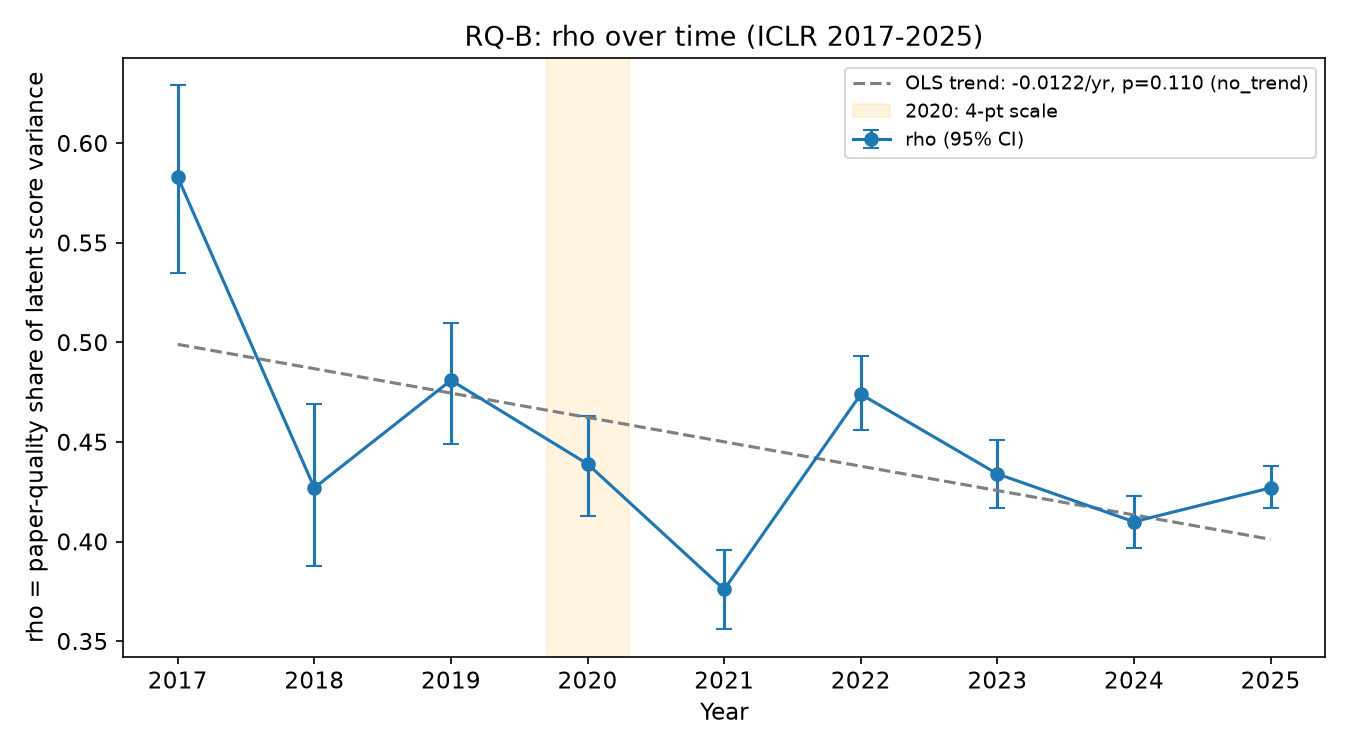
\includegraphics[width=0.85\textwidth]{fig_rho_trend.png}
\caption{RQ-B: $\rho$ over 2017--2025 with the OLS trend ($-0.0122$/year, $p=0.110$; no trend). The shaded band marks the 2020 four-point scale.}
\label{fig:rho-trend}
\end{figure}
\begin{figure}[t]
\centering
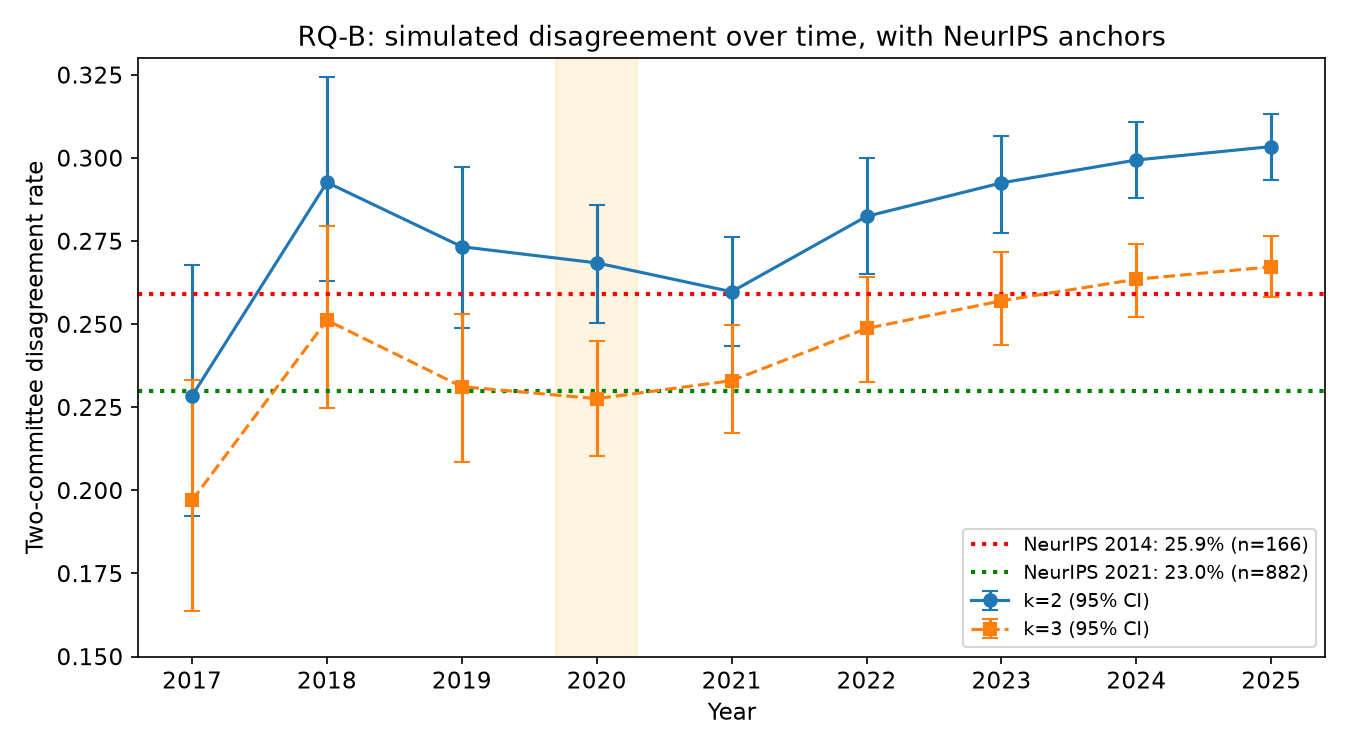
\includegraphics[width=0.85\textwidth]{fig_disagreement_trend.png}
\caption{RQ-B: simulated disagreement over 2017--2025 at $k=2$ and $k=3$ with the NeurIPS 2014 and 2021 anchors for reference. The nominal rise is not robust to dropping single years.}
\label{fig:disagreement-trend}
\end{figure}
A formal trend test of $\rho$ on year gives a slope of -0.0122 per year with p=0.110: no trend observed. A power calculation clarifies what this null means: with $n=9$, the design has 80\% power only for slopes of at least $\pm$0.022 per year (about $\pm$0.20 over the nine-year window), and power at the observed slope is 35\%. "No trend observed" is not "proof of no trend"; it is evidence against strong trends. Bivariate disagreement-on-year trends are nominally significant ($k=2$: +0.0062/year, p=0.028; $k=3$: +0.0065/year, p=0.008) but fragile: dropping 2017 raises the $k=2$ p-value to 0.147, and dropping any of 2023--2025 raises it to 0.052-0.080. Combined with the multivariate null, the conclusion is that there is no robust, attributable time trend in reviewer noise: the nominal 2017-to-2025 rise in $k=2$ disagreement (22.8\% to 30.3\%) cannot be separated into contributions from submission volume, reviewer counts, or scale changes.
%phase3_report.md sec 2.2
%phase3_report.md sec 2.2

\textbf{The 2020 and 2021 anomalies.} $P(\mathrm{flip}\mid\mathrm{accepted})$ at $k=2$ reaches 47.9\% in 2020 and 50.2\% in 2021, well above the 30-41\% range of the other years. Across years this quantity correlates -0.74 with $\rho$ and -0.83 with the acceptance rate (the two predictors are collinear; OLS on $n=9$ is not significant, $R^2$=0.70). The two years have different mechanisms.
%sim_summary.csv
%phase3_report.md sec 3.2

2020 used the four-point scale $\{1,3,6,8\}$, and the compression fingerprints are clear: 23.7\% of papers have zero within-paper score variance (versus 4.7-13.1\% in other years), score entropy is the lowest in the sample (1.27), and cutpoint spacing relative to the paper signal is the widest (1.67 sigma). Coarse scales quantize latent noise into whole-notch jumps: with $k=2$, a single reviewer moving one notch shifts the committee mean by 0.75 or more, making threshold crossings more likely.
%anomaly_descriptives.csv

\begin{figure}[t]
\centering
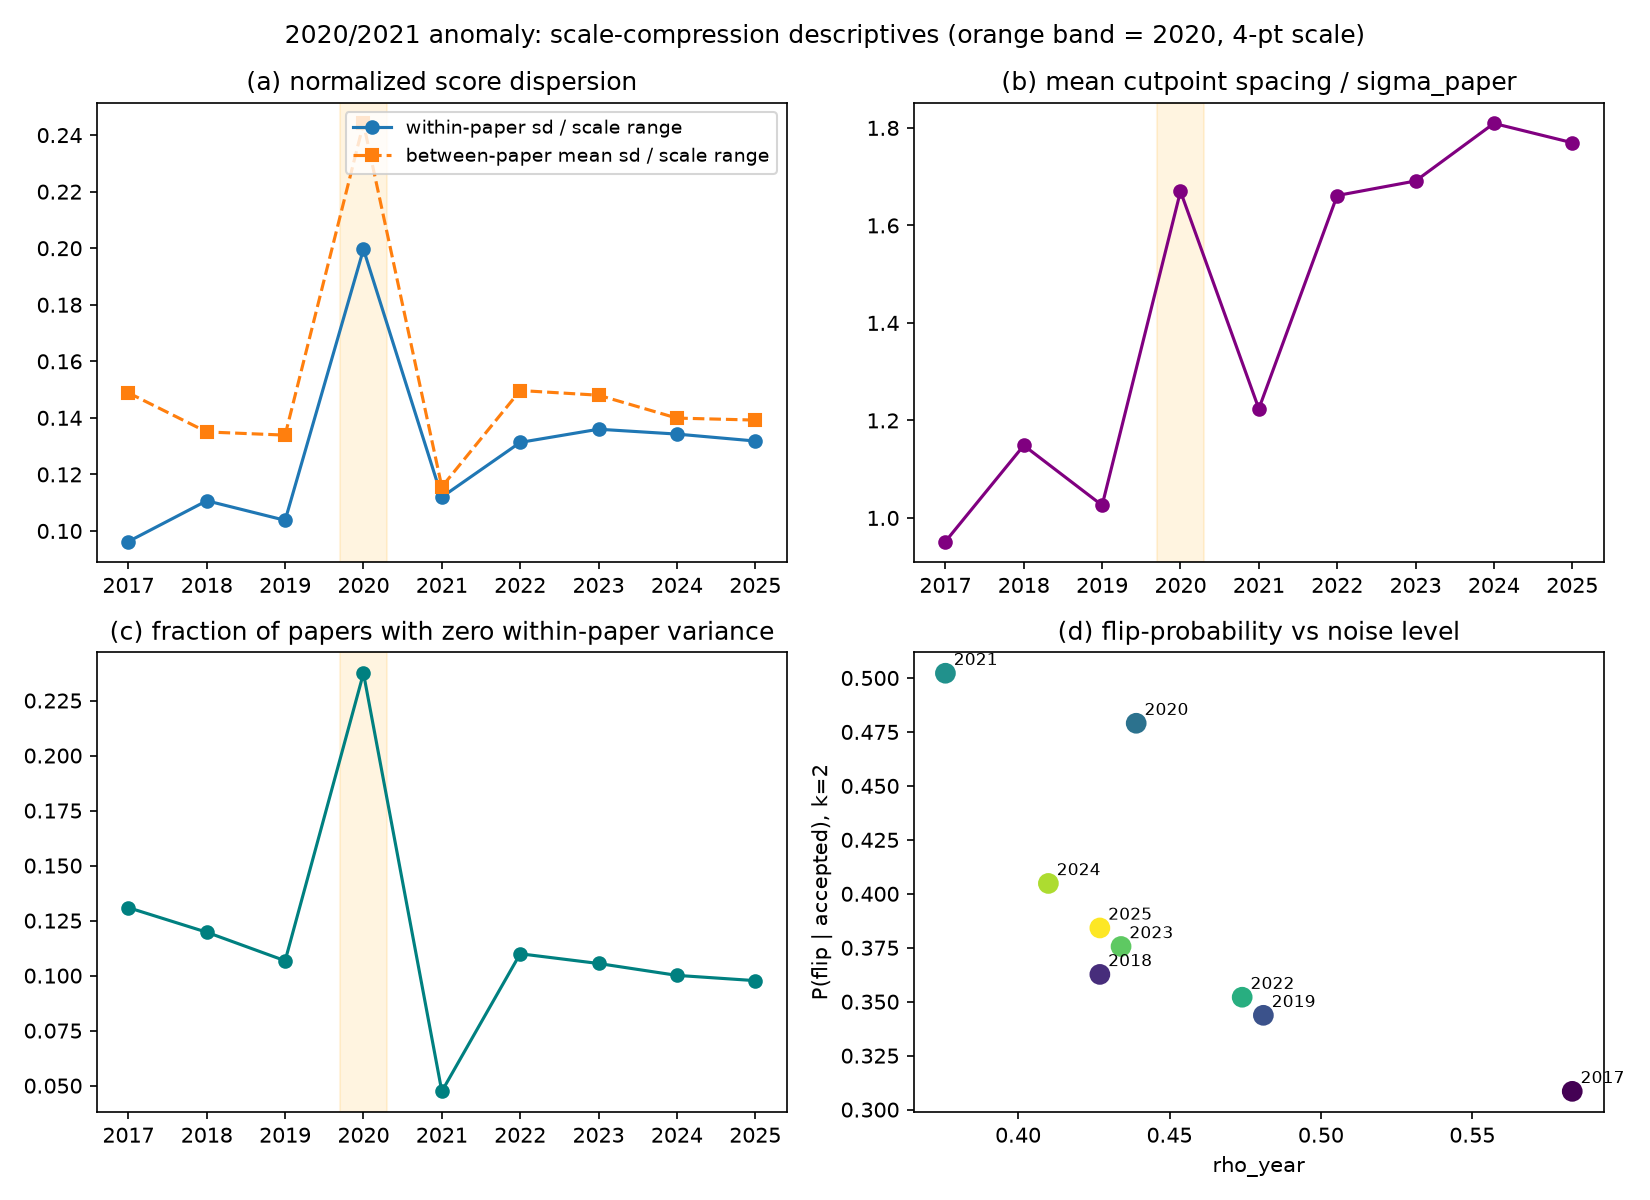
\includegraphics[width=0.95\textwidth]{fig_scale_compression.png}
\caption{2020/2021 anomaly descriptives. (a) Normalized score dispersion; (b) mean cutpoint spacing relative to $\sigma_{\mathrm{paper}}$; (c) fraction of papers with zero within-paper variance (23.7\% in 2020); (d) accepted-paper flip probability against $\rho$. The 2020 four-point scale (shaded) compresses scores; 2021 instead shows low signal with threshold crowding.}
\label{fig:scale-compression}
\end{figure}
2021 shows no compression fingerprint (zero-variance share is the nine-year minimum at 4.7\%). Its mechanism is low signal plus threshold crowding: $\rho$ is the sample minimum (0.376), and 30.4\% of accepted papers sit within 0.25 of the decision threshold (the sample maximum; median margin 0.50, the sample minimum). High noise with many acceptances hugging the threshold makes flips easy for a second committee.
%anomaly_descriptives.csv
%phase3_report.md sec 3.2

\textbf{Counterfactual: what does coarsening the scale do?} Mapping 2021's ten-point scores to the 2020 caliber $\{1,3,6,8\}$ by nearest neighbor, refitting the ordered probit (zero divergences), and re-simulating isolates the causal contribution of scale coarseness with cohort, year, and acceptance rate fixed. Quantization lowers $\rho$ from 0.376 [0.356, 0.396] to 0.345 [0.319, 0.369]: the coarse scale directly destroys about 8\% of the signal share, independent evidence of information loss. For comparability across the two worlds, decisions use a threshold rule with randomized tie-breaking calibrated so both worlds reproduce the empirical 33.1\% acceptance rate exactly (a fixed 0.5 logistic cutoff collapses the counterfactual acceptance rate to 9.9\%, so the logistic caliber is not comparable here). Coarsening the scale raises disagreement by about 7pp ($k=2$: 0.301 to 0.374) and $P(\mathrm{flip}\mid\mathrm{accepted})$ by about 11\,pp ($k=2$: 0.455 to 0.565), consistently across $k=2$, 3, and 4. This cross-validates against the observed data: 2020's actual $\rho$ (0.439) exceeds 2021's (0.376), i.e., 2020 had less latent noise, yet the coarse scale inflated its observed disagreement to 2021's level (0.268 vs 0.260) and pushed its accepted-paper flip rate higher (0.479).
%phase3_report.md sec 3.3
%phase3_report.md sec 3.3; counterfactual_2021_threshold.csv
%counterfactual_2021_threshold.csv
%rho_table.csv; sim_summary.csv

\begin{table}[t]
\centering
\caption{Counterfactual: 2021 scores quantized to the 2020 four-point caliber (threshold-rule decisions, acceptance rate fixed at 33.1\% in both worlds).}\label{tab:t5}
\begin{tabular}{lrrrrrrrr}\toprule
k & Disagreement, 10-pt & Disagreement, 4-pt & Delta & P(flip \ & accepted), 10-pt & P(flip \ & accepted), 4-pt & Delta \\
\midrule
2 & 0.301 & 0.374 & +0.073 & 0.455 & 0.565 & +0.110 \\
3 & 0.265 & 0.338 & +0.073 & 0.401 & 0.511 & +0.110 \\
4 & 0.239 & 0.308 & +0.069 & 0.361 & 0.465 & +0.104 \\
\bottomrule
\end{tabular}
\end{table}
% source: counterfactual_2021_threshold.csv

\subsection{RQ-C: the LLM era, descriptively}

The preregistration specified an interrupted time series at 2023 for within-paper score variance, review length, and confidence, plus an aggregate LLM-share estimate using the corpus-level method of Liang et al.~\citep{liang2024}. Two data constraints, both verified before analysis, reshaped this question (declared deviations): the primary data carry no review text (0 of 134,912 non-empty) and no confidence values, and the only review-text source (PeerSum, 53,732 reviews) ends in 2022. There are therefore no review-length or confidence data for 2023 or later, and the Liang et al. method, which requires post-ChatGPT review text corpora, is infeasible. Per the preregistered constraint against training a classifier or labeling individual reviews, no LLM-share estimate was attempted.
%phase1_report.md; llm_its.json
%preregistration_draft.md sec 3.7; llm_its.json

What can be reported is descriptive. An interrupted time series on normalized within-paper score variance over all nine years finds no break at 2023: level change +0.0099 (p=0.864), slope change -0.0026 (p=0.766). The design has almost no power for this test: at 80\% power it can only detect level jumps of $\pm$0.19 against a baseline variance of 0.01-0.04, i.e., five-to-tenfold changes. Dropping the anomalous 2020 still finds no break (level p=0.191, slope p=0.201), though the pre-2023 baseline slope itself is positive (+0.0012/year, p=0.031), meaning within-paper variance was slowly rising before 2023 without a jump at the breakpoint; 2023--2025 values are stable at 0.017-0.019.
%llm_its.json
%llm_its.json

\begin{figure}[t]
\centering
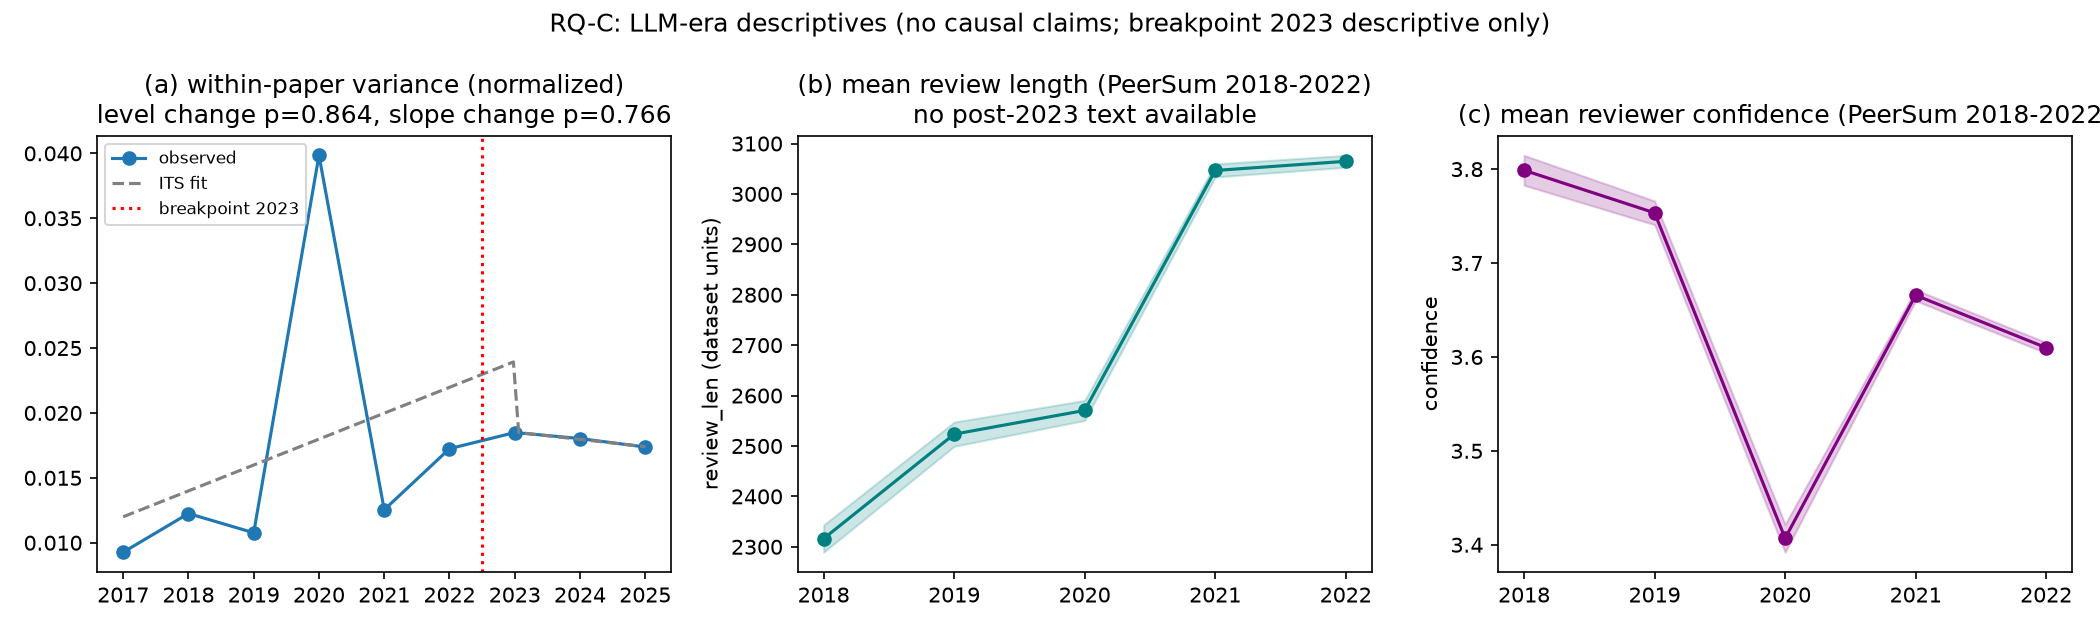
\includegraphics[width=0.95\textwidth]{fig_llm_descriptives.png}
\caption{RQ-C descriptives (no causal claims). (a) Within-paper score variance with a 2023 breakpoint (ITS: level $p=0.864$, slope $p=0.766$; near-zero power); (b) mean review length, PeerSum 2018--2022 only; (c) mean reviewer confidence, PeerSum 2018--2022 only. No post-2022 review text or confidence data exist.}
\label{fig:llm-descriptives}
\end{figure}
Review length (PeerSum, 2018--2022 only) rose about 32\% from 2018 to 2021 (mean 2,316 to 3,047 characters) and then flattened in 2022 (3,065); mean confidence is stable at 3.4-3.8 with median 4.0 every year. None of these behavioral proxies can be attributed to LLMs: they may reflect submission growth, process changes, or scale changes. The honest summary is that the data cannot support a conclusion about LLM effects on reviewing in either direction.
%llm_descriptives.csv

\section{Discussion}

\textbf{What the calibration buys.} The central methodological claim of this paper is modest: disagreement between two simulated committees, estimated from public scores alone, tracks two independent empirical targets within a few percentage points. The external target (23.0\% at NeurIPS 2021) is matched at +0.3\,pp under the matched reviewer-count caliber; the internal target, which assumes nothing about score generation, is matched within 1\,pp in the six most recent years. The preregistered worry, that omitting area-chair noise and reviewer-assignment variation would bias the estimator downward, is not borne out at the matched caliber; if anything the bias is mildly upward. A natural reading is that reviewer noise in the observed ICLR data already contains most of the assignment variation that a duplicated-review experiment would add. The practical consequence is that the "review lottery" can be audited cheaply and repeatedly: any conference that publishes scores and decisions can compute its own disagreement curve without running an experiment.

\textbf{Scale design matters.} The counterfactual experiment has the clearest policy implication among our results: coarsening the 2021 scores from ten points to four raises simulated disagreement by about 7pp and accepted-paper flips by about 11\,pp, holding everything else fixed. The 2020 four-point experiment at ICLR therefore did not merely re-label the same latent opinions; it measurably increased the randomness of outcomes. Conferences choosing coarse rubrics for simplicity should weigh this cost. Conversely, the 2021 anomaly shows that even a fine-grained scale does not protect against noise when the signal is weak and acceptances crowd the threshold: 2021 combined the lowest $\rho$ in the sample with the highest share of near-threshold acceptances, and half of its accepted papers would flip under a second committee.

\textbf{The long view.} Over nine years in which submissions grew $24$-fold, we find no robust trend in reviewer noise. That is a null result with limited power, not a clean bill of health, but it is the result the data support. It also echoes the NeurIPS 2021 experiment's own conclusion that inconsistency had not visibly changed since 2014 \citep{beygelzimer2023}. The review process, by this measure, is neither collapsing nor improving; it is persistently noisy at roughly the same level.

\textbf{On LLMs.} We report no finding about LLM effects on reviewing, and we consider that restraint a feature. The aggregate detection method we preregistered requires post-2022 review text that our public sources do not have. Behavioral proxies (review length up 32\% through 2021, then flat; confidence stable) move before any plausible LLM breakpoint and cannot be attributed. The literature's estimates (6.5-16.9\% of review text substantially LLM-modified at ICLR 2024 and peers; Liang et al., arXiv:2403.07183) come from corpora we do not have. Until post-2022 review text is available in public mirrors, the LLM question for ICLR remains open.

\section{Limitations}

\begin{enumerate}
\item \textbf{Longitudinal power.} With nine annual observations, the trend tests are weak: the $\rho$ trend test has 80\% power only for slopes of $\pm$0.022/year, and the RQ-C interrupted time series can only detect level jumps of $\pm$0.19 against a baseline of 0.01-0.04. The null results are honest zeros, not proof of stability.
\item \textbf{Collinearity.} Submission growth, the 2021 shift from three to four reviewers per paper, and scale changes occurred together (VIF about 5.8), so their contributions cannot be separated; the regression attributes nothing robustly to any of them.
\item \textbf{RQ-C is unattributable.} No post-2022 review text or confidence data exist in the public sources; the preregistered Liang et al. aggregate estimate was infeasible and was not attempted; no per-review AI classification was performed (also prohibited by the preregistration).
\item \textbf{Counterfactual scope.} The scale-coarsening experiment runs in one direction only (2021 to the 2020 caliber) and uses a threshold decision rule with randomized tie-breaking rather than the main logistic model, because the logistic caliber is not comparable across the two worlds (acceptance-rate collapse to 9.9\% versus 33.1\%). The effect size is therefore specific to the threshold-rule caliber, and the decision model extrapolates to "as if area chairs saw only coarse scores."
\item \textbf{Reviewer identities are unavailable.} Reviewer stringency cannot be estimated and is folded into the noise term; the model cannot distinguish a harsh reviewer from a noisy one. This was declared in the research plan.
\item \textbf{Partial external calibration.} The NeurIPS anchors are numerical comparisons, not refits: the public NeurIPS 2021 reviews cover accepted papers only, and the comparison matches reviewer-count calibers rather than re-running the full pipeline on NeurIPS data.
\item \textbf{Early-year internal gaps.} The $3$--$5$\,pp gaps between model and split-half anchor in 2017, 2019, and 2020 are explained by a hypothesis (reviewer-assignment homogeneity; coarser early scales), not by a test.
\item \textbf{ICLR only.} Cross-venue generalization was moved out of the main paper in the research plan; the estimator is validated on ICLR and NeurIPS anchors but applied only to ICLR.
\end{enumerate}

\section{Conclusion}

From public review data alone, we estimate that replacing the reviewer pool would flip the accept/reject decision for roughly one quarter of ICLR papers, and reject 30-50\% of currently accepted papers. The estimator survives two calibrations: it reproduces the NeurIPS 2021 experiment's 23.0\% disagreement within 0.3pp and matches a model-free split-half benchmark within 1\,pp in recent years. Over 2017--2025 we find no robust trend in reviewer noise despite $24$-fold submission growth. Rating-scale design has a measurable causal footprint: coarsening scores from ten points to four raises disagreement by about 7pp. The LLM era shows no detectable break in the behavioral proxies available, but the available data cannot address the question. The review lottery is real, it is stable, and it can now be audited without running an experiment.

\section{Appendix A. Claim-evidence checklist}

Each substantive claim in this draft maps to generated evidence. All tables and figures are produced by scripts in \texttt{scripts/}; paths are relative to \texttt{~/workspace/review-lottery/}.

\begin{table}[t]
\centering
\small
\caption{Claim-to-evidence checklist: each substantive claim maps to generated evidence.}\label{tab:claims}
\begin{tabular}{c p{5.2cm} p{5.2cm} p{3.2cm}}\toprule
\# & Claim & Evidence & Verdict \\
\midrule
1 & The estimator is externally calibrated: simulated disagreement matches NeurIPS 2021 (23.0\%) at the matched $k=3$ caliber & \texttt{phase2\_notes/calib\_external.csv}; \texttt{figures/fig\_calib\_external.png}; reported values in \texttt{phase0\_notes/papers.md} & Supported: bias +0.3\,pp \\
2 & The estimator agrees with a model-free internal anchor & \texttt{phase2\_notes/internal\_anchor.json}; \texttt{figures/fig\_calib\_internal.png} & Supported 2018, 2021--2025 (bias <1\,pp); early years $-3$ to $-5$\,pp, explained \\
3 & Rho is 0.38-0.58 across years, consistent with ~50\% subjective variation & \texttt{phase2\_notes/$\rho$\_table.csv}; \texttt{figures/fig\_$\rho$.png}; Cortes and Lawrence, arXiv:2109.09774 & Supported \\
4 & Two-committee disagreement is 23-30\% ($k=2$), 18-24\% ($k=4$); 30-50\% of accepted papers flip & \texttt{phase2\_notes/sim\_summary.csv} & Supported \\
5 & No robust longitudinal trend in reviewer noise, 2017--2025 & \texttt{phase3\_notes/regression\_results.json}; \texttt{phase3\_notes/longitudinal\_table.csv}; \texttt{figures/fig\_$\rho$\_trend.png}, \texttt{fig\_disagreement\_trend.png} & Supported (null result, low power declared) \\
6 & The 2020 anomaly is scale compression & \texttt{phase3\_notes/anomaly\_descriptives.csv}; \texttt{figures/fig\_scale\_compression.png} & Supported (descriptive fingerprints) \\
7 & Coarsening the scale causally raises disagreement (~+7\,pp) and accepted-paper flips (~+11\,pp) & \texttt{phase3\_notes/counterfactual\_2021\_threshold.csv}; \texttt{posteriors/draws\_2021\_q4.npz} & Supported, threshold-rule caliber; one-directional \\
8 & The 2021 anomaly is low $\rho$ plus threshold crowding & \texttt{phase3\_notes/anomaly\_threshold\_crowding.csv}; \texttt{phase2\_notes/$\rho$\_table.csv} & Supported (descriptive) \\
9 & No 2023 breakpoint in within-paper score variance & \texttt{phase3\_notes/llm\_its.json}; \texttt{figures/fig\_llm\_descriptives.png} & No break observed; power near zero (declared) \\
10 & Review length rose ~32\% (2018-2021), then flattened; confidence stable; no 2023+ data & \texttt{phase3\_notes/llm\_descriptives.csv}, \texttt{llm\_conf\_dist.csv} & Supported (descriptive only, no attribution) \\
11 & Aggregate LLM-share estimation (Liang et al.) not feasible & \texttt{phase3\_notes/llm\_its.json} ("liang\_method": "infeasible"); data audit in \texttt{phase1\_report.md} & Declared deviation, not attempted \\
12 & Data provenance and compliance (36,113 papers; 134,912 reviews; PII removed; no reviewer identities) & \texttt{phase1\_report.md}; \texttt{phase1\_notes/annual\_table.csv}; \texttt{scripts/01\_load\_clean.py} & Supported \\
13 & Confidence-term sensitivity: omitting $\beta\cdot\mathrm{conf}$ changes $\rho$ by -0.016 to -0.030 & \texttt{phase2\_notes/conf\_sensitivity.json}; \texttt{scripts/04b\_conf\_sensitivity.py} & Supported; declared deviation \\
\bottomrule
\end{tabular}
\end{table}


\begin{thebibliography}{9}
\bibitem[Beygelzimer et al.(2023)]{beygelzimer2023}
Alina Beygelzimer, Yann N. Dauphin, Percy Liang, Jennifer Wortman Vaughan. Has the Machine Learning Review Process Become More Arbitrary as the Field Has Grown? The NeurIPS 2021 Consistency Experiment. \textit{arXiv:2306.03262 [cs.LG]}, 2023. \url{https://arxiv.org/abs/2306.03262}

\bibitem[Cortes and Lawrence(2021)]{cortes2021}
Corinna Cortes, Neil D. Lawrence. Inconsistency in Conference Peer Review: Revisiting the 2014 NeurIPS Experiment. \textit{arXiv:2109.09774 [cs.DL]}, 2021. \url{https://arxiv.org/abs/2109.09774}

\bibitem[Liang et al.(2024)]{liang2024}
Weixin Liang et al. Monitoring AI-Modified Content at Scale: A Case Study on the Impact of ChatGPT on AI Conference Peer Reviews. \textit{arXiv:2403.07183 [cs.CL]}, 2024. \url{https://arxiv.org/abs/2403.07183}

\bibitem[Tran et al.(2020)]{tran2020}
David Tran et al. An Open Review of OpenReview: A Critical Analysis of the Machine Learning Conference Review Process. \textit{arXiv:2010.05137 [cs.LG]}, 2020. \url{https://arxiv.org/abs/2010.05137}

\bibitem[Process-centric(2025)]{acceptance2025}
What Drives Paper Acceptance? A Process-Centric Analysis of Modern Peer Review. \textit{arXiv:2509.25701}, 2025. \url{https://arxiv.org/abs/2509.25701}
\end{thebibliography}

\end{document}